% ============================================================
% Mechanistic Validity: A Framework and Automated Pipeline
% for Evaluating Interpretability Claims
% ============================================================
\pdfoutput=1
\documentclass[10pt]{article}
\usepackage[preprint]{tmlr}

\usepackage[T1]{fontenc}
\usepackage[utf8]{inputenc}
\usepackage{microtype}
\usepackage{amsmath,amssymb}
\usepackage{booktabs}
\usepackage{graphicx}
\usepackage{xcolor}
\usepackage{hyperref}
\usepackage{cleveref}
\usepackage{enumitem}
\usepackage{multirow}
\usepackage{array}
\usepackage{float}
\graphicspath{{figures/}}

\newcommand{\mechval}{\textsc{MechVal}}
\newcommand{\ie}{i.e.}
\newcommand{\eg}{e.g.}
\newcommand{\cf}{cf.}
\newcommand{\tighttable}{\setlength{\tabcolsep}{4pt}\renewcommand{\arraystretch}{1.05}}

\title{Mechanistic Validity: A Framework and Automated Pipeline for Evaluating Interpretability Claims}

\author{Elliot Tower \\
Independent Researcher \\
\texttt{elliot@elliottower.com}}

\begin{document}

\maketitle

% ============================================================
\begin{abstract}
Mechanistic interpretability lacks a shared standard for evaluating how well-supported a mechanistic claim actually is. We present \mechval{}, a measurement-theoretic framework that organizes 27 operational criteria across five validity types (construct, measurement, internal, external, interpretive) in dependency order, assigns claims to seven verdict tiers (five progressive tiers from Proposed through Validated, plus two lateral verdicts: Underdetermined and Disconfirmed), and supports evaluation via 58 metrics spanning five evidence families. The framework is method-agnostic, applying uniformly to circuits, SAE features, probing classifiers, steering vectors, transcoders, and crosscoders. We apply the framework manually to 13 published circuits, demonstrating that the tier system discriminates meaningfully: claims range from Proposed through Triangulated, with verdict differences traceable to specific missing evidence. To make the framework scalable, we present an automated evaluation pipeline that scores any MI paper on all 27 criteria in 2--3 minutes. Developed across 60+ configurations spanning 8 frontier models, the pipeline agrees with consensus reference labels on all 9 case-study papers to within one tier, matching exactly on 4. All disagreements are in the same direction---the system scores at most one tier too high, never too low---making its output a conservative upper bound on evidential quality.
\end{abstract}

% ============================================================
\section{Introduction}
\label{sec:intro}

When should you trust an interpretability claim? A researcher reports that GPT-2 uses a six-role circuit to solve indirect object identification \citep{wang2023interpretability}, that sparse autoencoder features correspond to human-interpretable concepts \citep{cunningham2023sparse}, or that a linear probe reveals syntactic structure in transformer activations \citep{belinkov2022probing}. Each claim comes with experimental evidence---ablation studies, activation visualizations, accuracy numbers. But how well-supported is the claim, really?

Recent work provides uncomfortable answers. \citet{bricken2024monosemanticity} and \citet{engels2025not} demonstrate that only 197 of 65,536 sparse autoencoder features---0.3\%---are stable across independent training runs. The remaining 99.7\% are training artifacts. Any ``deception feature'' identified using standard SAE methods has a 99.7\% prior probability of being an artifact, not a genuine representation.

The field's primary causal tool fares no better. \citet{kramar2024atp} show that attribution patching---the most widely used method for identifying causally relevant components---correlates at $r = 0.006$ with ground truth on controlled synthetic tasks. This is not a weak correlation; it is no correlation. The method that the field treats as the gold standard for causal attribution provides essentially random rankings of component importance.

The evaluation metrics used to assess these tools are themselves unreliable. The SAEBench audit subjects six standard SAE evaluation metrics to three diagnostic tests: reseed stability, ground-truth correlation, and discriminability. Two of six---Token Prediction Probability and Sparse Cross-entropy Recovery---fail all three diagnostics. Finally, the research itself does not reproduce. MechEvalAgent \citep{bai2026mecheval} performs execution-grounded evaluation of published MI research: 93\% of papers fail reproducibility checks when their code is actually run.

This paper contributes both halves of a solution. First, we propose \mechval{}, a measurement-theoretic framework that synthesizes validation methodology from philosophy of science, neuroscience, psychometrics, pharmacology, and causal inference (\Cref{sec:framework}--\Cref{sec:foundations}). The framework defines 27 operational criteria, 5 verdict tiers, 5 evidence families, and a \texttt{MechanisticClaimSpec} data model that supports pre-registration of mechanistic hypotheses. We apply it manually to 13 published circuits, demonstrating that the tier system discriminates meaningfully (\Cref{sec:case-studies}). Second, because manual application takes hours per paper, we present an automated evaluation pipeline that operationalizes the framework end-to-end (\Cref{sec:pipeline}). The pipeline completes a full paper evaluation in 2--3 minutes and agrees with human-adjudicated reference labels on 9 papers to within one tier (\Cref{sec:results}).

% ============================================================
\section{Related Work}
\label{sec:related}

Existing structured evaluations of MI focus narrowly. MIB \citep{mueller2025mib} defines a benchmark for circuit localization and causal-variable localization but does not evaluate the full evidential basis of a claim. MechEvalAgent \citep{bai2026mecheval} audits MI papers for execution-grounded reproducibility---whether their code runs and produces the claimed numbers---finding 93\% failure. Our framework is complementary: rather than asking whether a paper's code reproduces, we ask whether the paper's evidence supports its mechanistic conclusion.

The LLM-as-evaluator paradigm has demonstrated that large language models can serve as effective judges for open-ended tasks \citep{zheng2024judging}. Known failure modes include positional bias, verbosity bias, and over-charitable interpretation. The automated pipeline we present inherits these limitations and explicitly characterizes them; our directional-asymmetry finding (the system over-scores by at most one tier, never under-scores) is consistent with the over-charitable-interpretation literature.

The framework draws on five established validation traditions: Popperian falsifiability and severe testing \citep{mayo2018statistical}; lesion studies and double dissociation from neuroscience; construct, convergent, and discriminant validity from psychometrics; dose-response and assay calibration from pharmacology; and necessity, sufficiency, and transportability from causal inference \citep{pearl2009causality, pearl2011transportability}. The contribution is not any one of these---it is their integration into a single dependency-ordered protocol for MI claims.

% ============================================================
\section{The \mechval{} Framework}
\label{sec:framework}

\subsection{Five Validity Types in Dependency Order}
\label{sec:validity-types}

The framework organizes evaluation into five validity types, applied in dependency order:
%
\begin{equation}
\text{Construct} \rightarrow \text{Measurement} \rightarrow \text{Internal} \rightarrow \text{External} \rightarrow \text{Interpretive}
\label{eq:dependency}
\end{equation}
%
Each type depends on the validity of the types before it. A measurement of an ill-defined construct is meaningless; a causal inference from an unreliable measurement is meaningless; a generalization claim from an untested causal inference is meaningless.

\textbf{Construct validity} asks whether the thing being measured is well-defined. Before any measurement is taken, the construct must be specified precisely enough that the claim is falsifiable and structurally plausible. A ``deception feature'' that cannot be distinguished from an ``uncertainty feature'' fails construct validity regardless of how carefully it is measured.

\textbf{Measurement validity} asks whether the metrics are trustworthy. Once the construct is defined, the measurement tools must be reliable (stable across repetitions), calibrated (separable from random baselines), and invariant (consistent across conditions). A metric that gives different answers when run with different random seeds is not evidence.

\textbf{Internal validity} asks whether the evidence supports the causal claim. The evidence must establish that the identified component is causally involved in the behavior---not merely correlated with it. This requires demonstrating necessity, sufficiency, and specificity.

\textbf{External validity} asks whether the mechanism generalizes. Causal evidence on one prompt set, with one ablation method, in one model, establishes internal validity at best. External validity requires generalization across prompts, ablation methods, related tasks, and ideally across models.

\textbf{Interpretive validity} asks whether the interpretation is correct. The natural-language description of the mechanism must be justified by the evidence. A head called a ``name mover'' based on direct logit attribution carries theoretical implications beyond what the evidence strictly supports.

\begin{figure}[t]
\centering
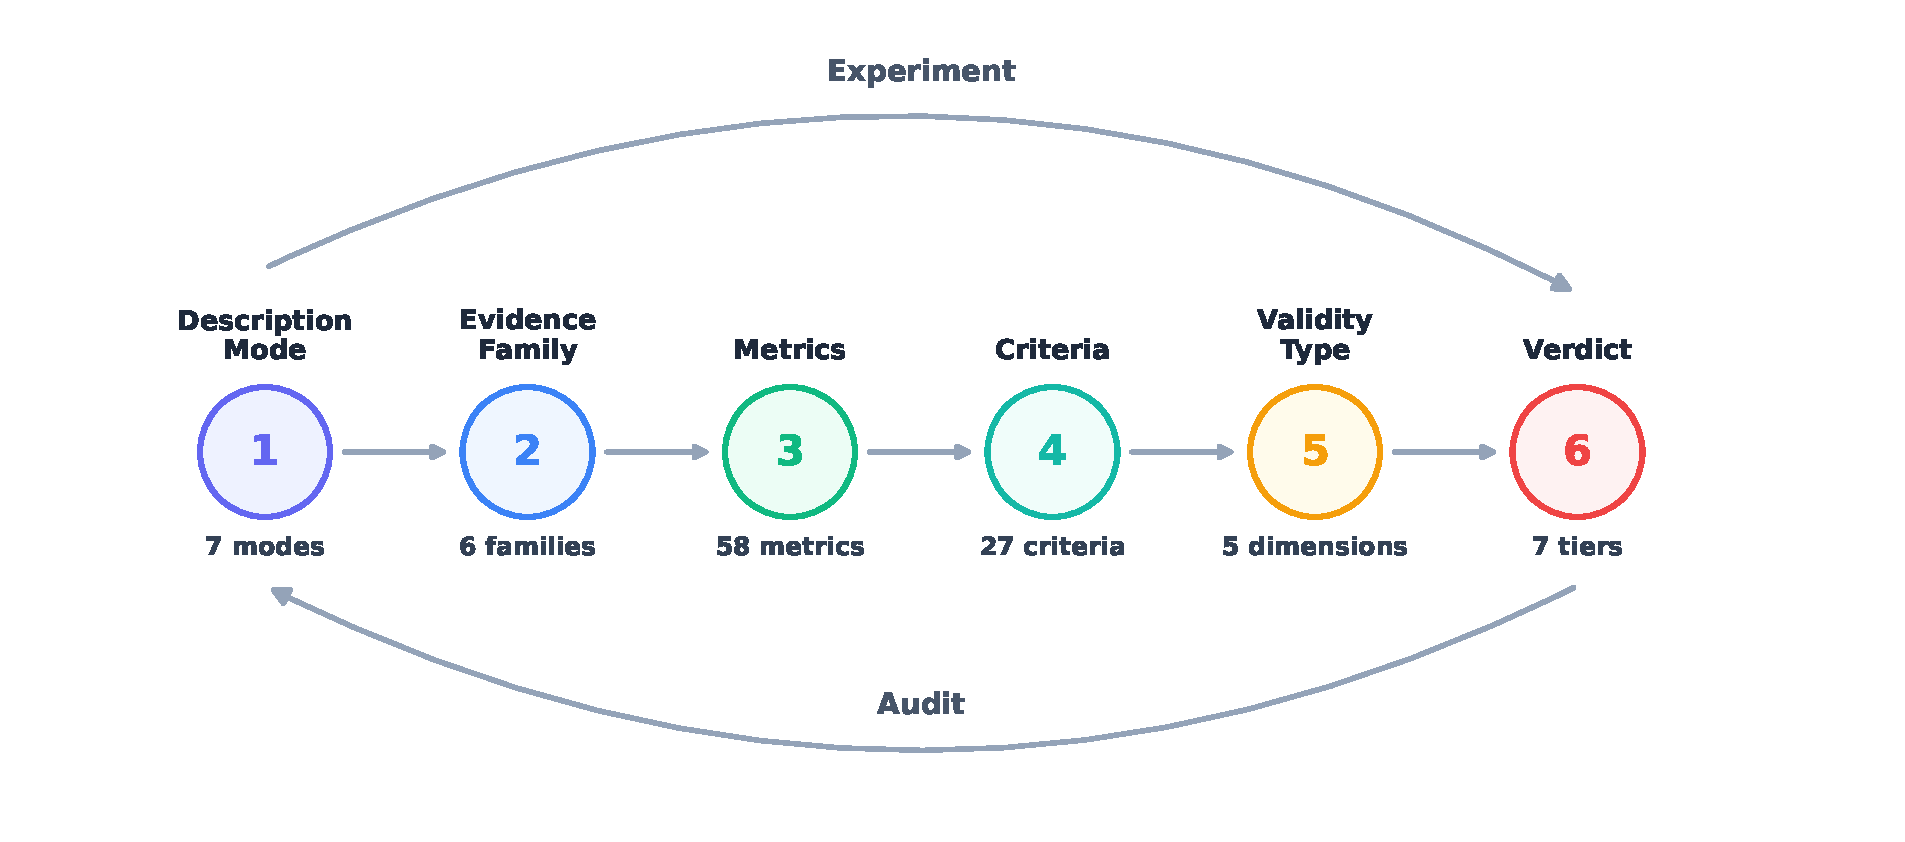
\includegraphics[width=\linewidth]{pipeline-final.pdf}
\caption{The \mechval{} framework hierarchy. Six layers from description mode through verdict. \textbf{Experiment} (top, left-to-right): from raw measurements, build upward through criteria and validity types to a verdict. \textbf{Audit} (bottom, right-to-left): given a claimed verdict, trace backward to identify which lower-layer criteria are unmet.}
\label{fig:pipeline}
\end{figure}

\subsection{Twenty-Seven Criteria}
\label{sec:criteria}

Each validity type is operationalized through specific criteria, totaling 27 across the five types (\Cref{tab:criteria}). Each criterion has a concrete test: a claim either passes, partially passes, or fails each criterion, producing a structured validity profile rather than a single score.

\begin{table}[t]
\centering
\tighttable
\caption{The 27 operational criteria organized by validity type.}
\label{tab:criteria}
\small
\begin{tabular}{@{}llp{7.5cm}@{}}
\toprule
\textbf{Type} & \textbf{ID} & \textbf{Criterion} \\
\midrule
\multirow{5}{*}{Construct} & C1 & Falsifiability --- can the claim be refuted? \\
& C2 & Structural plausibility --- is the mechanism physically possible in the architecture? \\
& C3 & Task specificity --- is the mechanism specific to the claimed task? \\
& C4 & Minimality --- are all components necessary, with no redundant members? \\
& C5 & Convergent validity --- do multiple independent methods agree? \\
\midrule
\multirow{5}{*}{Internal} & I1 & Necessity --- is the circuit required for the behavior? \\
& I2 & Sufficiency --- is the circuit enough to produce the behavior? \\
& I3 & Specificity --- does the circuit do this task and not everything? \\
& I4 & Consistency --- does the finding hold across samples, methods, and seeds? \\
& I5 & Confound control --- are alternative explanations ruled out? \\
\midrule
\multirow{6}{*}{Measurement} & M1 & Reliability --- do repeated measurements give the same answer? \\
& M2 & Invariance --- does the metric behave consistently across conditions? \\
& M3 & Baseline separation --- is the score distinguishable from random baselines? \\
& M4 & Sensitivity --- can the metric detect known-true effects? \\
& M5 & Calibration --- are the numbers meaningful and interpretable? \\
& M6 & Construct coverage --- does the metric measure its nominal target? \\
\midrule
\multirow{6}{*}{External} & E1 & Intervention reach --- do different intervention methods agree? \\
& E2 & Graded response --- does partial ablation produce partial effects? \\
& E3 & Selectivity --- does the intervention affect the target but not other tasks? \\
& E4 & Effect magnitude --- are the effects large enough to support the claim? \\
& E5 & Robustness --- does the claim survive perturbation and varied conditions? \\
& E6 & Cross-architecture --- does the mechanism appear in other model families? \\
\midrule
\multirow{5}{*}{Interpretive} & V1 & Level declaration --- at what description mode is the claim made? \\
& V2 & Level-evidence match --- does the evidence support claims at that level? \\
& V3 & Narrative coherence --- does the paper tell a consistent mechanistic story? \\
& V4 & Alternative exclusion --- are competing explanations considered and addressed? \\
& V5 & Scope honesty --- does the claim acknowledge its limitations? \\
\bottomrule
\end{tabular}
\end{table}

\subsection{Evidence Families}
\label{sec:evidence-families}

Metrics are organized into five evidence families, each providing a different kind of evidence about a mechanistic claim:

\begin{itemize}[nosep]
    \item \textbf{Causal:} Effects of interventions---ablation, patching, clamping, resampling. Examples: activation patching, DAS-IIA, CATE, mediation analysis.
    \item \textbf{Structural:} Weight-space properties, requiring no forward pass. Examples: SVD, effective rank, OV/QK composition norms, template distance.
    \item \textbf{Information-theoretic:} Information flow and dependencies. Examples: mutual information, partial information decomposition, transfer entropy.
    \item \textbf{Behavioral:} Input-output behavior under manipulation. Examples: faithfulness, logit difference, KL divergence, dose-response curves.
    \item \textbf{Representational:} Geometry and content of internal representations. Examples: CKA, RSA, linear probes, attention entropy.
\end{itemize}

The distinction between families matters because convergent evidence---the same conclusion supported by metrics from different families---is qualitatively stronger than redundant evidence from the same family. An ablation study (causal) that agrees with a weight-space analysis (structural) provides more support than two ablation studies using different ablation methods.

\subsection{Verdict Tiers}
\label{sec:verdict-tiers}

Claims are assigned to one of seven verdicts. Five form a strict hierarchy representing qualitative transitions in evidential status (\Cref{tab:verdicts}); two are \emph{lateral} verdicts that sit outside the progression.

\begin{table}[t]
\centering
\tighttable
\caption{Verdict tiers with requirements. The five progressive tiers form a strict hierarchy; each subsumes the requirements of all lower tiers. Two lateral verdicts (Underdetermined, Disconfirmed) sit outside the progression.}
\label{tab:verdicts}
\small
\begin{tabular}{@{}lp{4.2cm}p{5.5cm}@{}}
\toprule
\textbf{Verdict} & \textbf{Meaning} & \textbf{Requirements beyond previous tier} \\
\midrule
\multicolumn{3}{@{}l}{\textit{Progressive tiers}} \\
Proposed & Structural or representational evidence only & Construct validity criteria met (C1--C5) \\
Causally Suggestive & Necessity shown, sufficiency not established & Internal validity I1 (necessity via ablation) \\
Mech.\ Supported & Necessity + sufficiency with consistent methods & I1 + I2 (sufficiency), intervention reach (E1), at least 2 ablation variants \\
Triangulated & Multiple converging lines of independent evidence & Full internal + external + construct criteria from $\geq 3$ evidence families \\
Validated & All five validity types addressed & Measurement + interpretive validity with explicit baselines \\
\midrule
\multicolumn{3}{@{}l}{\textit{Lateral verdicts}} \\
Underdetermined & Evidence consistent with multiple competing accounts & Named rival hypotheses; no available experiment distinguishes them \\
Disconfirmed & Evidence actively contradicts the claim & Prediction failure, artifact demonstration, or construct dissolution \\
\bottomrule
\end{tabular}
\end{table}

The progressive tier system is designed to be informative at every level. A Proposed claim is not invalid---it is a claim whose evidential status is precisely characterized. The verdict tells researchers exactly what additional evidence would advance the claim: a Proposed claim needs causal intervention (I1) to reach Causally Suggestive; a Causally Suggestive claim needs sufficiency evidence (I2) and method consistency (E1) to reach Mechanistically Supported.

The two lateral verdicts capture conclusions that do not fit on the evidential ladder. \textbf{Underdetermined} applies when the evidence is consistent with multiple mechanistic accounts and no available experiment distinguishes them---the claim is not wrong, but the evidence does not select between competing explanations. \textbf{Disconfirmed} applies when evidence actively contradicts the claim: a specific prediction fails, the mechanism is shown to be a measurement artifact, or the construct dissolves under scrutiny. Disconfirmation is not failure---it is informative, narrowing the space of possible mechanisms.

\subsection{Description Modes}
\label{sec:description-modes}

MI claims operate at different levels of description, following Marr's hierarchy adapted for transformer circuits. The framework defines six description modes forming a partial order by evidential commitment: computational (what function, why), algorithmic (what procedure), representational (what information, in what geometry), implementational-functional (what each component does), implementational-connectomic (how components are wired), and implementational-topographic (which components are involved). Higher modes require all evidence from lower modes plus bridging evidence connecting levels.

\subsection{\texttt{MechanisticClaimSpec}: Pre-Registration}
\label{sec:claimspec}

The framework's primary original contribution is a Pydantic v2 data model that encodes a mechanistic hypothesis \emph{before} verification. A \texttt{MechanisticClaimSpec} specifies computational steps (nodes in the mechanism DAG mapped to specific model components), directed edges (specifying communication mechanisms), positive predictions (testable claims about what should happen under intervention), negative controls (claims about what should not happen), rival specifications (competing hypotheses), and gate metadata (identifiability and superposition risk assessments).

When \texttt{verify(spec)} runs, it executes each prediction by routing to the appropriate metric, compares measured values against expected directions and thresholds, and aggregates results into a confirmation rate, negative control rate, claim ceiling, and verdict tier. The pre-registration requirement prevents post-hoc rationalization---the practice of discovering a circuit and then constructing a narrative that fits the observations without ever testing predictions the narrative would make.

% ============================================================
\section{Theoretical Foundations}
\label{sec:foundations}

The framework synthesizes validation methodology from five established fields. \Cref{tab:crossfield} maps framework components to their cross-field analogs.

\subsection{Philosophy of Science}

The construct validity criteria (C1--C5) draw on Popper's falsifiability criterion, Mayo's severe testing \citep{mayo2018statistical}, and Glennan's new mechanical philosophy \citep{glennan2017new}. C1 requires that a mechanistic claim state what evidence would disprove it---a requirement routinely violated in MI, where circuit labels are often applied post-hoc without pre-registered predictions. C5 (convergent validity) requires that the claim be supported by multiple independent methods, following Campbell and Fiske's multitrait-multimethod matrix. The verdict tier system mirrors the hierarchy of evidential support in philosophy of science: observation (Proposed), single-method causal evidence (Causally Suggestive), multi-method causal evidence (Mechanistically Supported), convergent evidence from independent methods (Triangulated), and comprehensive evaluation (Validated).

\subsection{Neuroscience}

The internal validity criteria (I1--I5) are adapted from neuroscience's toolkit for establishing that a neural circuit implements a computation. I1 (necessity) corresponds to lesion studies: removing the circuit disrupts the behavior. I2 (sufficiency) corresponds to stimulation: activating the circuit alone produces the behavior. I3 (specificity) mirrors the logic of double dissociation in neuropsychology---showing that the component does this task and not everything. The critical distinction between necessity and sufficiency---well-established in neuroscience but often elided in MI---is central to the framework. Most published circuits demonstrate necessity but not sufficiency. The framework treats this distinction as a qualitative transition between verdict tiers.

\subsection{Psychometrics}

The measurement validity criteria (M1--M6) draw on psychometric principles of test construction. M1 (reliability) is test-retest reliability: the same metric applied to the same model should give the same answer. M2 (invariance) is measurement invariance: the metric should behave consistently across conditions. M3 (baseline separation) operationalizes the basic psychometric requirement that a score must exceed chance to be meaningful. The calibration gates (F01--F15 in the implementation) operationalize these principles as concrete statistical tests.

\subsection{Pharmacology}

The external validity criteria, particularly E2 (graded response), draw on pharmacology's dose-response methodology. A causally relevant component should produce graded effects: partial ablation should produce partial behavioral change, and the relationship should be monotonic or at least systematic. The framework treats dose-response as a minimum bar for causal claims about magnitude---a requirement absent from most MI evaluations, which typically report binary ablation (all-or-nothing). The three-phase protocol used in the case studies mirrors the phase structure of clinical trials.

\subsection{Causal Inference}

The benchmark architecture is grounded in causal inference methodology \citep{pearl2009causality, spirtes2000causation}. Track~1 (Circuit Localization) corresponds to causal discovery. Track~2 (Causal Variable Localization) corresponds to causal abstraction \citep{geiger2023causal}. Track~3 (Causal Model Testing) corresponds to model testing in the Pearl framework---testing whether a proposed causal model is consistent with interventional data. This track is the framework's primary original contribution---theory-driven hypothesis testing rather than blind discovery.

\begin{table}[t]
\centering
\tighttable
\caption{Cross-field mapping of framework components to established methodology.}
\label{tab:crossfield}
\small
\begin{tabular}{@{}lp{2.0cm}p{2.0cm}p{2.0cm}p{1.8cm}p{2.0cm}@{}}
\toprule
\textbf{Component} & \textbf{Causal Inf.} & \textbf{Neuroscience} & \textbf{Psychometrics} & \textbf{Pharma.} & \textbf{Phil.\ of Sci.} \\
\midrule
Track 1 & Causal discovery & Circuit mapping & Exploratory FA & Target discovery & Abduction \\
Track 2 & Causal abstraction & Functional localization & Construct oper. & Target charac. & Natural kinds \\
Track 3 & Model testing & Circuit dissection & Confirmatory FA & Proof of mech. & H-D testing \\
V1 & ATE/CATE & Perturbation quant. & Effect size est. & Dose-response & Parameter est. \\
V2 & Transportability & Cross-condition gen. & Meas.\ invariance & Phase III gen. & Novel prediction \\
\bottomrule
\end{tabular}
\end{table}

% ============================================================
\section{Case Studies: Thirteen Published Circuits}
\label{sec:case-studies}

We apply the framework manually to 13 published MI results, evaluating each through all five validity lenses. The case studies demonstrate what the framework looks like in practice and show that the tier system discriminates between well-validated and poorly-validated claims.

% ------ Figure 2 placeholder ------
% FIGURE 2: Tier assignment overview — horizontal bar chart or matrix showing
% the 13 circuits arranged by tier (Proposed → Triangulated), with colored
% cells indicating which validity dimensions are satisfied/partial/unsatisfied.

\subsection{Verdict Assignments}

\Cref{tab:case-studies} presents the verdict assignments. The key finding is that the tier system produces meaningful discrimination: the 13 claims span the full range from Proposed to Triangulated, with verdict differences traceable to specific missing evidence rather than arbitrary scoring.

\begin{table}[t]
\centering
\tighttable
\caption{Verdict assignments for 13 published circuits, based on published evidence as of evaluation date.}
\label{tab:case-studies}
\small
\begin{tabular}{@{}llp{6.5cm}@{}}
\toprule
\textbf{Verdict} & \textbf{Circuit} & \textbf{Key limiting criterion} \\
\midrule
\multirow{3}{*}{Triangulated} & Induction Heads & Broad replication across scales; thick evidential network \\
& Grokking & All criteria met within toy scope; tier-capped (no real-model evidence) \\
& Superposition & All criteria met in toy models; tier-capped (no real-model evidence) \\
\midrule
\multirow{3}{*}{\parbox{2.3cm}{Mechanistically\\Supported}} & IOI Circuit & Method-conditional faithfulness (87\% mean ablation, $<$50\% other methods); specificity untested \\
& Greater-Than & Strong structural plausibility (C2); limited prompt generalization \\
& Copy Suppression & Unusually clean specificity; sufficiency partially established \\
\midrule
\multirow{5}{*}{\parbox{2.3cm}{Causally\\Suggestive}} & Successor Heads & Cross-domain generalization as convergent evidence; ablation method-conditional \\
& Docstring Circuit & Label ambiguity: ``variable binding'' vs.\ simpler ``positional copying'' \\
& SAE Features & Features may be dictionary properties, not model properties \\
& Othello World Model & ``World model'' label exceeds evidence; interpretive inflation \\
& Knowledge Neurons & Strong intervention but weak mechanistic story; construct clarity \\
\midrule
\multirow{2}{*}{Proposed} & Probing Classifiers & Decodability without intervention $=$ no internal validity \\
& Gender Bias Circuits & Construct incoherence: bias and knowledge share circuits \\
\bottomrule
\end{tabular}
\end{table}

\subsection{Illustrative Examples}

\paragraph{Induction Heads (Triangulated).} \citet{olsson2022context} identify a two-head composition mechanism for in-context copying: previous-token heads attend to the token before a repeated sequence, and induction heads use this signal to predict the next token. The claim reaches Triangulated because it satisfies criteria across multiple independent evidence families. The mechanism has been replicated across model scales and architectures (E6), confirmed through both activation-level and weight-level analysis (C5, convergent validity from different families), and produces clean dose-response effects (E2). The relative simplicity of the mechanism makes each criterion easier to satisfy.

\paragraph{IOI Circuit (Mechanistically Supported).} \citet{wang2023interpretability} identify 26 attention heads forming a six-role circuit for indirect object identification. The circuit demonstrates strong necessity (I1) and sufficiency (I2): running the model with everything outside the circuit mean-ablated recovers 87\% of the full model's logit difference. However, \citet{miller2024transformer} show that this 87\% figure is specific to mean ablation; under other ablation methods, faithfulness drops below 50\%. This method-conditional result partially satisfies E1 (intervention reach) but reveals that the causal claim is weaker than the headline number suggests. Specificity (I3) is untested: the authors do not report whether ablating the IOI circuit degrades unrelated tasks. The circuit reaches Mechanistically Supported rather than Triangulated because the evidence comes primarily from one methodological family and key criteria (I3, I4, I5, E6) remain unaddressed.

\paragraph{Probing Classifiers (Proposed).} Linear probing \citep{belinkov2022probing} trains a classifier on activations to test whether a concept is linearly decodable. The core limitation is fundamental: \emph{a measurement without an intervention is a measurement without internal validity}. Probe success establishes that information is decodable from the activation space, but not that the model uses that information during inference. Without causal follow-up, the claim cannot advance beyond Proposed. The framework does not dismiss probing---it precisely characterizes what probing alone does and does not establish.

\subsection{Patterns Across Case Studies}

\paragraph{The sufficiency gap.} Most circuits demonstrate necessity (I1) but not sufficiency (I2). The I1$\rightarrow$I2 transition is the most common barrier between Causally Suggestive and Mechanistically Supported.

\paragraph{Method-conditional results.} The IOI circuit's headline numbers are specific to mean ablation. Ablation type is part of the causal claim, not an implementation detail. The framework captures this through E1 (intervention reach).

\paragraph{The toy-model tier cap.} Grokking and Superposition satisfy nearly all criteria within their toy-model scope, but the framework caps toy-model-only results at Triangulated---the Validated tier requires evidence from real pretrained models. Both reach Triangulated rather than Validated, illustrating that completeness within a restricted scope is a genuine achievement (not a failure) while honestly representing the gap to real-model confirmation.

\paragraph{Interpretive inflation.} Labels like ``world model,'' ``knowledge neuron,'' and ``deception feature'' carry theoretical implications beyond what the evidence supports. The framework identifies this through V4 (alternative exclusion) and V5 (scope honesty).

% ============================================================
\section{Automated CVS Pipeline}
\label{sec:pipeline}

Manual application of the framework takes hours per paper. To make the framework deployable across the literature, we built an automated pipeline that takes any MI paper as input and produces a Claim Validity Score (CVS) and verdict tier in 2--3 minutes.

% ------ Figure 3 placeholder ------
% FIGURE 3: Pipeline architecture diagram. Four stages:
% (1) Text extraction (PDF/HTML → text)
% (2) 3× independent LLM extraction (claims + 27 criteria each)
% (3) Multi-run minimum voting (per criterion)
% (4) Evidence audit (separate LLM call, no paper text)
% → Dimension scores → CVS → Tier

\subsection{Pipeline Architecture}

Given a paper from any supported source (arXiv, OpenReview, PDF URL, blog post, or local file), the system performs four stages:

\begin{enumerate}[nosep]
    \item \textbf{Text extraction} --- PDF parsing via pypdf (50-page limit) or HTML scraping for blog posts.
    \item \textbf{Multi-run claim extraction} --- three independent LLM calls, each extracting mechanism claims and scoring all 27 criteria as YES (1.0), PARTIAL (0.5), or NO (0.0).
    \item \textbf{Multi-run minimum voting} --- for each (claim $\times$ criterion) cell, the minimum across the three runs is retained.
    \item \textbf{Evidence audit} --- a separate LLM call receives the scored claims \emph{without the paper text} and checks whether circuit-level evidence was incorrectly attributed to sub-component claims.
\end{enumerate}

The pipeline then computes dimension scores from the criteria and a final CVS on a normalized 0--10 scale.

\subsection{Criteria Assessment}

Each claim is scored on all 27 criteria using the framework's definitions (\Cref{tab:criteria}). The extraction prompt includes 10 explicit scoring pitfalls drawn from common errors observed during development:

\begin{enumerate}[nosep]
    \item Faithfulness metrics do not establish sufficiency (I2 requires isolation or path-level tests).
    \item Template variation does not equal cross-task testing (same task, different names $=$ E1, not E3).
    \item Same architecture, different size does not equal cross-architecture (GPT-2 Small vs.\ Medium $\neq$ E6).
    \item Activation patching and path patching count as a single method for convergent validity (C5).
    \item Probing is correlational --- no internal validity from probes alone.
    \item Most papers do not declare description mode; if inferred, V1 $=$ NO.
    \item IIA without random baseline $=$ M3 NO.
    \item Ablation establishes necessity only --- do not give I2 from ablation.
    \item Negative results count for specificity (I3).
    \item Controls often live in the appendix --- read it.
\end{enumerate}

When scoring a sub-component claim, only experiments that directly test the components in that claim count---evidence from experiments on other components does not transfer. This is what the evidence audit enforces post-hoc.

\subsection{Dimension Aggregation}
\label{sec:aggregation}

Raw criteria are aggregated into dimension scores (0--3) using validity-theoretic rules that encode domain knowledge about what constitutes strong versus weak evidence. These rules use logical conjunctions rather than averages, reflecting the fact that certain criteria are prerequisites for higher scores.

For \textbf{construct validity}, a score of 3 requires all five criteria satisfied ($\sum \geq 5.0$). A score of 2 requires convergent validity (C5 $\geq$ YES) and aggregate score $\geq 3.0$. A score of 1 requires any criterion satisfied ($\sum \geq 1.0$). A score of 0 indicates no construct evidence.

For \textbf{internal validity}, a score of 3 requires necessity (I1), sufficiency (I2), specificity (I3), and confound control (I5). A score of 2 requires both necessity and sufficiency. A score of 1 requires either alone. These thresholds reflect the MI community's consensus that necessity (ablation) and sufficiency (circuit isolation) are the two pillars of causal mechanistic evidence.

For \textbf{measurement validity}, scoring is gated on baselines: a score of 3 requires a random baseline (M3 $=$ YES), reliability (M1), calibration (M5), and sensitivity (M4). A score of 2 requires random baseline and reliability. A score of 1 requires any baseline comparison. This reflects the observation that many MI papers compare only to the full model, providing limited information about whether the reported effect exceeds chance.

For \textbf{external validity}, a score of 3 requires cross-architecture validation (E6 $\geq$ YES) and strong aggregate evidence ($\sum \geq 4.0$). A score of 2 requires cross-architecture or selectivity (E3 $\geq$ YES). A score of 1 requires intervention reach (E1 $\geq$ PARTIAL).

For \textbf{interpretive validity}, scoring is based on aggregate evidence, with scores of 3 ($\sum \geq 4.0$), 2 ($\geq 2$ sub-criteria at PARTIAL and $\sum \geq 2.5$), or 1 ($\sum \geq 1.0$).

\subsection{CVS Computation and Tier Classification}

The Claim Validity Score is a weighted sum of dimension scores, normalized to a 0--10 scale:
%
\begin{equation}
\text{CVS} = \frac{\sum_{d \in D} w_d \cdot s_d}{\sum_{d \in D} 3 \cdot w_d} \times 10
\end{equation}
%
where $s_d \in \{0,1,2,3\}$ is the dimension score and $w_d$ is the dimension weight. Construct and internal validity receive weight 1.5; measurement, external, and interpretive validity each receive weight 1.0. The maximum raw score is 18.0, yielding a CVS of 10.0.

Tier boundaries: Proposed ($<2.0$), Causally Suggestive ($2.0$--$3.9$), Mechanistically Supported ($4.0$--$5.9$), Triangulated ($6.0$--$7.9$), Validated ($\geq 8.0$).

\subsection{Multi-Run Minimum Voting}

Run-to-run variance in LLM scoring introduces significant noise: the same paper can score between 5.6 and 6.9 across identical extraction runs with temperature 0, due to non-deterministic GPU kernel execution. This variance is asymmetric---the model sometimes awards YES on borderline criteria stochastically, but rarely awards NO on criteria that genuinely deserve YES.

Multi-run minimum voting exploits this asymmetry. The system runs $N=3$ independent extractions, then for each criterion takes the minimum status using the ordering NO $<$ PARTIAL $<$ YES. The approach is conservative by design: it can only reduce scores, never inflate them.

\subsection{Evidence Audit}

A key failure mode in automated extraction is \emph{evidence misattribution}: a sub-component claim is credited with evidence that actually describes a larger circuit. Consider the IOI paper: ``87\% faithfulness'' measures the full 26-head circuit running in isolation, not any individual head group. But when the extraction LLM encounters this number while scoring the Name Mover heads (a 3-head subset), it tends to award sufficiency (I2) based on evidence that does not apply at that granularity.

The evidence audit catches this with a second-pass API call that receives the scored claims \emph{without the paper text}. The auditor sees only each claim's description and the short evidence strings the extractor attached to each criterion---no surrounding context from the paper. For each of five criteria empirically prone to misattribution (I2, I3, I5, E2, E5), the auditor makes a binary decision: does this evidence string actually describe an experiment on the components named in this claim? If not, the criterion is downgraded. System-level claims (describing the whole circuit) are never downgraded, since circuit-level evidence is in scope for circuit-level claims.

\subsection{Worked Example: IOI Name Mover Heads}

We trace one IOI claim through the full pipeline. The claim: \emph{``Name Mover heads (9.9, 9.6, 10.0) copy the indirect object token from earlier positions to the final token position.''}

\textbf{Initial extraction.} C1 $=$ YES (specific heads, testable operation). I1 $=$ YES (ablation degrades performance). I2 $=$ YES (evidence: ``87\% faithfulness''). E2 $=$ YES (``gradual degradation curve'').

\textbf{Multi-run minimum ($N=3$).} I2 receives YES/YES/PARTIAL across runs. Minimum: PARTIAL.

\textbf{Evidence audit.} The auditor sees the claim (``Name Mover heads 9.9, 9.6, 10.0'') and the evidence string (``87\% faithfulness''). That faithfulness number describes the 26-head circuit, not the 3-head subset---the evidence is out of scope. I2 downgraded from PARTIAL to NO. E2's ``gradual degradation'' similarly comes from circuit-level ablation; E2 downgraded from YES to NO.

\textbf{Final scoring.} Construct $= 2$, Internal $= 1$ (necessity only), Measurement $= 1$, External $= 0$, Interpretive $= 2$. CVS $= (1.5 \cdot 2 + 1.5 \cdot 1 + 1.0 \cdot 1 + 1.0 \cdot 0 + 1.0 \cdot 2) / 18.0 \times 10 = 4.2$, reduced to 3.9 after audit-driven downgrades---appropriately lower than the main circuit claim's 5.6.

% ============================================================
\section{Experimental Results}
\label{sec:results}

\subsection{Model Comparison}

We evaluated the pipeline across 8 frontier language models and 60+ configurations spanning extraction architecture (one- to three-step), reasoning modes, and 15 prompt iterations. \Cref{tab:models} shows performance on the IOI paper.

% ------ Figure 4 placeholder ------
% FIGURE 4: Model comparison scatter plot. X-axis: model name/config.
% Y-axis: main claim CVS. Horizontal band showing the reference tier
% (Mech. Supported, 4.0-5.9). Points colored by thinking mode.

\begin{table}[t]
\centering
\tighttable
\caption{Model comparison on IOI (main claim CVS). Reference: Mech.\ Supported (5.6).}
\label{tab:models}
\small
\begin{tabular}{@{}llcccc@{}}
\toprule
\textbf{Model} & \textbf{Thinking} & \textbf{Claims} & \textbf{Main CVS} & \textbf{Predicted Tier} & \textbf{Off-by} \\
\midrule
Claude Opus 4.7 & Off & 8 & 5.6 & Mech.\ Supported & 0 \\
DeepSeek V4 Pro & High & 9 & 5.6 & Mech.\ Supported & 0 \\
DeepSeek V4 Pro & Max & 7 & 5.6 & Mech.\ Supported & 0 \\
GPT-5.5 & Off & 9 & 6.4 & Triangulated & +1 \\
GPT-5.5 & On & 10 & 6.4 & Triangulated & +1 \\
Claude Opus 4.7 & High & 9 & 6.9 & Triangulated & +1 \\
Gemma 4 27B & --- & 5 & 7.5 & Triangulated & +1 \\
Qwen 3.7 Max & Thinking & 7 & 7.5 & Triangulated & +1 \\
GPT-5.4 Mini & --- & 10 & 8.3 & Validated & +2 \\
Qwen 3.7 Max & Off & 8 & 8.1 & Validated & +2 \\
GLM-5.1 & --- & 0 & --- & Failed & --- \\
\bottomrule
\end{tabular}
\end{table}

Enabling chain-of-thought reasoning consistently worsened calibration: Claude Opus 4.7 scores exactly right with thinking off (5.6) but over-scores with thinking enabled (6.9). We hypothesize that chain-of-thought amplifies the model's charitable-interpretation prior---the model reasons itself into higher scores.

\subsection{Headline Result}

\Cref{tab:results} presents the main results with multi-run minimum debiasing ($N=3$).

% ------ Figure 5 placeholder ------
% FIGURE 5: Results bar chart. 9 papers on Y-axis, CVS on X-axis.
% Bar color = predicted tier. Black diamonds = expected tier midpoint.
% Shows all errors above diagonal (over-scoring only).

\begin{table}[t]
\centering
\tighttable
\caption{Final results with multi-run minimum + evidence audit. All errors are $+1$ (over-scoring); no papers are under-scored.}
\label{tab:results}
\small
\begin{tabular}{@{}lccllc@{}}
\toprule
\textbf{Paper} & \textbf{CVS} & \textbf{N claims} & \textbf{Predicted Tier} & \textbf{Expected Tier} & \textbf{Off-by} \\
\midrule
Probing & 1.4 & 3 & Proposed & Proposed & 0 \\
Gender Bias & 3.3 & 5 & Caus.\ Suggestive & Proposed & +1 \\
Successor Heads & 3.1 & 4 & Caus.\ Suggestive & Caus.\ Suggestive & 0 \\
Greater-Than & 5.6 & 5 & Mech.\ Supported & Caus.\ Suggestive & +1 \\
Othello & 4.4 & 3 & Mech.\ Supported & Caus.\ Suggestive & +1 \\
IOI & 5.6 & 5 & Mech.\ Supported & Mech.\ Supported & 0 \\
Copy Suppression & 5.6 & 4 & Mech.\ Supported & Mech.\ Supported & 0 \\
Induction & 6.4 & 4 & Triangulated & Mech.\ Supported & +1 \\
Grokking & 8.3 & 5 & Validated & Triangulated & +1 \\
\bottomrule
\end{tabular}
\end{table}

Of the 9 evaluated papers, 4 received the exact expected tier (44\%) and all 9 were within one tier (100\%). All 5 disagreements are in the $+1$ direction---the system never under-scores. The Grokking over-score reflects a tier cap: the pipeline scores it at Validated by CVS, but toy-model-only results are capped at Triangulated. We note that $N=9$ is a small evaluation set; these results should be interpreted as a case study characterizing the system's tendencies rather than a precise accuracy benchmark.

\subsection{Directional Asymmetry as Conservative Upper Bound}

The error distribution is markedly asymmetric: 4 over-scored, 0 under-scored. This pattern is consistent across all 60+ configurations, all 8 models, and both debiased and undebiased conditions. It is a structural property of LLM-as-judge applied to MI papers, not stochastic noise.

Two error sources drive the residual bias. First, the model awards YES on borderline criteria where PARTIAL or NO would be more accurate---particularly I3 (specificity), E2 (graded response), and I5 (confound control). Second, over-scoring concentrates at the Causally Suggestive / Mechanistically Supported boundary. Third, the pipeline does not yet enforce the toy-model tier cap, contributing one additional +1 error (Grokking: predicted Validated, expected Triangulated).

This asymmetry is exploitable. Because the system never under-scores, its output functions as a \emph{certified upper bound} on evidential quality. A paper rated Mechanistically Supported might actually be Causally Suggestive; a paper rated Proposed cannot be hiding a higher true tier. For literature triage---``which papers are worth manually validating?''---this is exactly the property you want.

\subsection{Debiasing Effectiveness}

Multi-run minimum voting improves the single-run baseline (2/9 exact matches, max off-by $+2$ on Greater-Than) to 4/9 exact matches with no paper off by more than 1 tier. The improvement is most pronounced for papers near tier boundaries, where a single generous criterion judgment can push the score into the next tier.

The evidence audit reduced mean absolute per-criterion error from 0.163 to 0.111 on the IOI paper against 189-cell reference annotations (7 claims $\times$ 27 criteria). Per-criterion exact agreement improved from approximately 74.8\% to 81.5\%.

A devil's advocate challenge pass was tested as an alternative debiasing strategy. The aggressive version over-corrected (IOI from 6.9 to 4.2---one tier below consensus). A conservative version had no effect. This Goldilocks problem makes devil's advocate unreliable; we recommend multi-run minimum + evidence audit as the sole debiasing configuration.

% ------ Figure 6 placeholder ------
% FIGURE 6: Debiasing effect. Two panels:
% (a) Variance collapse: for each paper, show CVS range across 3 single
%     runs (red bar) and the multi-run minimum (green diamond).
% (b) Confusion matrix: predicted vs. expected tier (5×5 grid).
%     All errors above diagonal.

\subsection{Theoretical-Paper Limitation}

The Superposition paper \citep{elhage2022superposition} was excluded from the main evaluation. Its purely analytical methodology maps poorly onto criteria designed for empirical circuit-discovery papers. The pipeline scores it at Proposed (correctly, given it lacks real-model evidence) but the criteria driving that score are not the meaningful ones for a theory paper. Extending the system to handle theoretical papers without cross-contaminating empirical scoring remains an open challenge.

% ============================================================
\section{Discussion}
\label{sec:discussion}

\subsection{Pre-Registration and Post-Hoc Rationalization}

The \texttt{MechanisticClaimSpec} is the framework's most consequential design choice. It changes the unit of MI research from ``interesting finding'' to ``tested prediction.'' A claim that exists only as paper-text description can always be re-narrated to fit new evidence. A claim encoded as a Pydantic spec with positive predictions and negative controls cannot---\texttt{verify(spec)} returns numerical confirmation rates whether the author wants it to or not.

The IOI paper, the Greater-Than paper, and the Docstring paper would all benefit from being re-expressed as claim specs---not because their authors did anything wrong, but because the pre-registration discipline distinguishes which conclusions the evidence actually establishes from which conclusions were narrative additions.

\subsection{Implications for AI Safety}

The measurement crisis has direct deployment implications. Organizations are beginning to build internal monitors based on MI findings---probes that flag potential deception, steering vectors that suppress harmful outputs, circuit-level classifiers that trigger human review. If those monitors are built on unvalidated features, they provide false confidence: the system appears monitored when it is not.

The verdict tier system provides deployment guidance: Proposed features should not be deployed as monitors; Causally Suggestive features provide preliminary evidence only; Mechanistically Supported features have the minimum evidential basis for cautious deployment with ongoing validation. The automated pipeline extends this to the literature scale: an organization can apply the system to every published MI claim relevant to their safety case and produce a calibrated upper bound on which claims meet their deployment threshold.

\subsection{Limitations}

\paragraph{Manual case studies are based on published evidence only.} No novel model interventions were run for the 13-circuit analysis. The verdict assignments are arguments from published evidence, not experimental results. Running the framework's verification pipeline on all 12 claim specifications is future work pending GPU compute.

\paragraph{Automated pipeline scores are conservative upper bounds.} The $+1$ directional bias means the system over-states evidential quality on borderline cases. Users should treat the output as ``this paper is at most tier X.''

\paragraph{Reference label reliability.} The 9-paper consensus labels were established through multi-model voting plus human adjudication. A formal inter-annotator agreement study would be needed to establish definitive accuracy. We acknowledge a circularity concern: LLM extractions informed some reference labels, so the evaluation partly measures self-consistency rather than accuracy against fully independent ground truth. Four papers have registry-derived labels that predate the automated system.

\paragraph{Coverage gaps.} Of the 54 implemented evaluation tasks, only 12 have full claim specifications. The framework's utility grows with circuit coverage, which is bottlenecked by the labor-intensive process of circuit discovery and specification.

\paragraph{LLM-as-evaluator limitations.} Positional bias, verbosity bias, and over-charitable interpretation are present and characterized but not eliminated. We do not claim the automated pipeline replaces human review---only that it produces a calibrated triage signal.

\subsection{Future Work}

Running \texttt{verify(spec)} end-to-end on all 12 claim specifications with actual model interventions would replace manual case-study verdicts with experimentally-derived ones. Cross-checking framework verdicts against independent MIB benchmark scores would provide external validation. Cross-model ensembling---running extraction with multiple LLMs and retaining only criteria with consensus---could address the consistent over-scoring that multi-run minimum cannot fix. Expanding from 9 to 50+ reference papers with independent multi-annotator labels would enable more robust calibration.

% ============================================================
\section{Conclusion}
\label{sec:conclusion}

The mechanistic interpretability field has made remarkable progress in identifying circuits, features, and representations in neural networks. But progress in discovery has outpaced progress in validation. The result is a field that generates claims faster than it can evaluate them, using tools whose reliability is uncertain, producing results that do not reproduce.

The \mechval{} framework addresses this gap by providing the measurement infrastructure the field lacks. The 27 criteria, five validity types, five evidence families, and seven verdict tiers provide a common language for evaluating MI claims---whether they concern circuits, SAE features, probes, or steering vectors. The framework's application to 13 published circuits demonstrates that the tier system discriminates meaningfully. The automated CVS pipeline closes the deployment gap, bringing hours-per-paper evaluation down to minutes, with a calibrated directional bias that makes its output a useful conservative upper bound.

The framework is open-source and method-agnostic. Its contribution is a public good: the measurement infrastructure that makes interpretability claims trustworthy.

% ============================================================
\section*{Acknowledgments}

The framework draws on insights from the mechanistic interpretability community, particularly open problems identified by Sharkey et al.\ (2026) and the actionability framework of Orgad et al.\ (2026). The cross-field methodology benefits from established validation traditions in philosophy of science \citep{mayo2018statistical}, neuroscience, psychometrics, pharmacology, and causal inference \citep{pearl2009causality}.

% ============================================================
\bibliographystyle{tmlr}

\begin{thebibliography}{99}

\bibitem[Bai et~al.(2026)]{bai2026mecheval}
Bai, X., Baumgartner, T., Sun, C., Holtzman, A., and Tan, C.
\newblock MechEvalAgent: Execution-grounded evaluation of mechanistic interpretability research.
\newblock \emph{Preprint}, 2026.

\bibitem[Belinkov(2022)]{belinkov2022probing}
Belinkov, Y.
\newblock Probing classifiers: Promises, shortcomings, and advances.
\newblock \emph{Computational Linguistics}, 48(1):207--219, 2022.

\bibitem[Bricken et~al.(2024)]{bricken2024monosemanticity}
Bricken, T., Templeton, A., Batson, J., et~al.
\newblock Towards monosemanticity: Decomposing language models with dictionary learning.
\newblock \emph{Transformer Circuits Thread}, 2024.

\bibitem[Cunningham et~al.(2023)]{cunningham2023sparse}
Cunningham, H., Ewart, A., Riggs, L., Huben, R., and Sharkey, L.
\newblock Sparse autoencoders find highly interpretable features in language models.
\newblock \emph{arXiv:2309.08600}, 2023.

\bibitem[Elhage et~al.(2022)]{elhage2022superposition}
Elhage, N., Hume, T., Olsson, C., et~al.
\newblock Toy models of superposition.
\newblock \emph{Transformer Circuits Thread}, 2022.

\bibitem[Engels et~al.(2025)]{engels2025not}
Engels, J., Liao, I., Michaud, E.~J., Gurnee, W., and Tegmark, M.
\newblock Not all language model features are linear.
\newblock In \emph{NeurIPS}, 2025.

\bibitem[Geiger et~al.(2023)]{geiger2023causal}
Geiger, A., Wu, Z., Lu, H., et~al.
\newblock Causal abstraction: A theoretical foundation for mechanistic interpretability.
\newblock \emph{JMLR}, 2023.

\bibitem[Glennan(2017)]{glennan2017new}
Glennan, S.
\newblock \emph{The New Mechanical Philosophy}.
\newblock Oxford University Press, 2017.

\bibitem[Kr{\'a}m{\'a}r et~al.(2024)]{kramar2024atp}
Kr{\'a}m{\'a}r, J., Lieberum, T., Shah, R., and Neel, N.
\newblock Relevance propagation for transformers.
\newblock In \emph{NeurIPS}, 2025.

\bibitem[Mayo(2018)]{mayo2018statistical}
Mayo, D.~G.
\newblock \emph{Statistical Inference as Severe Testing}.
\newblock Cambridge University Press, 2018.

\bibitem[Miller et~al.(2024)]{miller2024transformer}
Miller, J., et~al.
\newblock Transformer circuit faithfulness metrics are not robust.
\newblock \emph{arXiv preprint}, 2024.

\bibitem[Mueller et~al.(2025)]{mueller2025mib}
Mueller, S., et~al.
\newblock The Mechanistic Interpretability Benchmark.
\newblock \emph{arXiv preprint}, 2025.

\bibitem[Olsson et~al.(2022)]{olsson2022context}
Olsson, C., Elhage, N., Nanda, N., et~al.
\newblock In-context learning and induction heads.
\newblock \emph{Transformer Circuits Thread}, 2022.

\bibitem[Pearl(2009)]{pearl2009causality}
Pearl, J.
\newblock \emph{Causality}.
\newblock Cambridge University Press, 2nd edition, 2009.

\bibitem[Pearl \& Bareinboim(2011)]{pearl2011transportability}
Pearl, J. and Bareinboim, E.
\newblock Transportability of causal and statistical relations: A formal approach.
\newblock In \emph{AAAI}, 2011.

\bibitem[Spirtes et~al.(2000)]{spirtes2000causation}
Spirtes, P., Glymour, C., and Scheines, R.
\newblock \emph{Causation, Prediction, and Search}.
\newblock MIT Press, 2nd edition, 2000.

\bibitem[Wang et~al.(2023)]{wang2023interpretability}
Wang, K., Variengien, A., Conmy, A., Shlegeris, B., and Steinhardt, J.
\newblock Interpretability in the wild: A circuit for indirect object identification in {GPT}-2 Small.
\newblock In \emph{ICLR}, 2023.

\bibitem[Zheng et~al.(2024)]{zheng2024judging}
Zheng, L., Chiang, W.-L., Sheng, Y., et~al.
\newblock Judging {LLM}-as-a-judge with {MT}-Bench and Chatbot Arena.
\newblock In \emph{NeurIPS}, 2024.

\end{thebibliography}

% ============================================================
% APPENDICES
% ============================================================
\appendix

\section{Full Per-Paper Results}
\label{app:results}

\textbf{IOI Circuit}: Main circuit claim 5.6 (Mech.\ Supported), Name Movers 3.9 (Caus.\ Suggestive), S-Inhibition 3.3 (Caus.\ Suggestive), Duplicate Token / Induction 3.3 (Caus.\ Suggestive), Backup Name Movers 3.3 (Caus.\ Suggestive).

\textbf{Grokking}: Modular addition algorithm 8.3 (Validated), Fourier components 1.9 (Proposed), MLP neurons 3.3 (Caus.\ Suggestive), Attention heads 1.9 (Proposed), Phase transition 2.5 (Caus.\ Suggestive).

\textbf{Copy Suppression}: Main L10H7 mechanism 5.6 (Mech.\ Supported), sub-claims 1.4--4.7.

\textbf{Probing}: All three claims scored 1.4 (Proposed).

\textbf{Successor Heads}: Main claim 3.1 (Caus.\ Suggestive), MLP0 1.9 (Proposed), Mod-10 features 4.7 (Mech.\ Supported), Pythia-1.4B 2.5 (Caus.\ Suggestive).

\textbf{Greater-Than}: Main circuit 5.6 (Mech.\ Supported), MLP contributions 3.3, Attention heads 3.3, MLP 10 neurons 3.3, Generalization 4.7.

\textbf{Induction}: Main induction head claim 6.4 (Triangulated), phase change 3.1, abstract ICL 1.4, smeared-key 1.4.

\textbf{Othello}: Board state 4.4 (Mech.\ Supported), causal link 4.4, nonlinear probes 3.1.

\textbf{Gender Bias}: Gender direction 3.3 (Caus.\ Suggestive), linear separability 1.9, hard debiasing 1.9, gender projection 0.0, indirect bias 0.0.

\section{Prompt Engineering Details}
\label{app:prompts}

The extraction prompt (v15b) contains approximately 3,500 tokens of criteria guidance organized into four sections: criteria-specific guidance for all 27 criteria, 10 scoring pitfalls, evidence scope rules, and theoretical paper guidance. A complete few-shot example presents a hypothetical subject-verb agreement circuit paper with appropriate scoring differentiation between circuit-level and sub-component claims. The evidence audit prompt contains approximately 500 tokens targeting the five misattribution-prone criteria (I2, I3, I5, E2, E5).

\section{Implementation Scale}
\label{app:scale}

The open-source implementation provides 54 evaluation tasks across 10 linguistic domains, 58 metrics spanning 5 evidence families (32 causal, 18 structural, 9 information-theoretic, 20 behavioral, 5 representational), 14 calibration gates, and 12 pre-registered \texttt{MechanisticClaimSpec}s covering circuits of varying complexity (IOI: 6 steps, 15 heads, 7 predictions, 5 negative controls; Greater-Than: 3 steps, 7 heads; Induction: 2 steps, 7 heads; and 9 others).

% ============================================================
% FIGURE PLAN (not rendered — for author reference)
% ============================================================
%
% Figure 1 (§3.1): Validity dependency chain
%   Five nodes (C → M → I → E → V) connected by arrows.
%   Below each node: one-line failure mode example.
%   Style: clean schematic, no photos.
%   Purpose: makes the dependency argument visual and memorable.
%
% Figure 2 (§5): Case study tier overview
%   Horizontal stacked bar or heatmap: 13 circuits on Y-axis,
%   5 validity dimensions as columns, cells colored by
%   satisfied/partial/unsatisfied. Rows grouped by tier.
%   Purpose: shows discrimination at a glance.
%
% Figure 3 (§6): Pipeline architecture
%   Left-to-right flow: Paper → Text Extraction → 3× LLM Extraction
%   → Min Voting → Evidence Audit → Dimension Scores → CVS → Tier.
%   Each stage labeled with API call count (4 total).
%   Purpose: makes the pipeline concrete and countable.
%
% Figure 4 (§7.2): Model comparison
%   Dot plot or bar chart: models on Y-axis, CVS on X-axis.
%   Reference band (4.0-5.9 = Mech. Supported) shaded.
%   Points colored by thinking mode (off/high/max).
%   Purpose: shows thinking hurts calibration.
%
% Figure 5 (§7.3): Main results
%   Bar chart: 9 papers on Y-axis sorted by expected tier.
%   Two marks per paper: predicted CVS (bar) and expected tier midpoint (diamond).
%   Purpose: headline result visualization.
%
% Figure 6 (§7.4): Debiasing effect
%   (a) For each paper: red range bar (single-run CVS range) plus
%       green diamond (multi-run minimum). Shows variance collapse.
%   (b) 5×5 confusion matrix (predicted vs expected tier).
%       All errors above diagonal.
%   Purpose: shows multi-run minimum eliminates stochastic component.
%
\end{document}
